\chapter{Splitting complex lawns}
\label{ch:split}

The passes of Chapter~\ref{ch:swaths} work best when they all run from one
side of the region to the other, with their ends lined up. On the L-shape
they did not: half of the passes stopped at the inner corner, and the order
with jumps sent the mower from one arm to the other. Around a hole, a line
meets the region twice, and a single set of passes cannot be driven one
after the other at all. This chapter cuts the interior into \emph{cells},
each of which is mowed by its own passes, in its own direction.

\section{Monotone regions}

\begin{definition}{Monotone region}{monotone}
  A region is \emph{monotone} in the direction $\theta$ if every line
  parallel to $\theta$ meets it in at most one segment.
\end{definition}

In a monotone region, every swath of Definition~\ref{def:swath} is a single
segment, so the passes of Chapter~\ref{ch:swaths} cover it and every turn
joins two passes at the same side. A convex region is monotone in every
direction. The interior of the L-shape is monotone in the direction of
either arm; the rectangle with a pond of Figure~\ref{fig:decomposition} is
monotone in no direction, since every line through the pond meets the
region on both sides of it.

\section{The boustrophedon decomposition}

In the frame where $\theta$ points along the $x$ axis, call the lines
parallel to $\theta$ \emph{horizontal}. The boustrophedon decomposition of
Choset~\cite{choset2000} (``boustrophedon'', as the ox turns at the end of
the furrow) cuts a polygon with holes into monotone cells in two steps.

\begin{description}
  \item[Cut.]
    \leavevmode\\
    Cut the polygon by the horizontal line through each of its vertices.
    Between two consecutive lines, the polygon falls into pieces.
  \item[Merge.]
    \leavevmode\\
    Going up from strip to strip, add a piece to the cell below it when
    each is the only neighbour of the other across the line between them;
    otherwise, start a new cell.
\end{description}

\begin{proposition}{Pieces are trapezoids}{trapezoids}
  Each piece of a strip between two consecutive vertex lines is a trapezoid
  with two horizontal sides; it is convex, hence monotone.
\end{proposition}

\begin{proof}
  No vertex of the polygon lies strictly between the two lines, so every
  edge of the boundary that enters the open strip crosses it from one line
  to the other. These edges do not cross each other and are ordered from
  left to right along any horizontal line of the strip; going along such a
  line, one enters and leaves the polygon each time one crosses an edge. A
  piece is therefore bounded by two consecutive edges, on its left and on
  its right, and by the two lines: a trapezoid.
\end{proof}

\begin{proposition}{Merging keeps monotone cells}{merge}
  Let $A$ be a monotone cell whose top is on the line $y = c$ and $B$ a
  monotone piece whose bottom is on the same line. If $B$ is the only piece
  above that line touching $A$, and $A$ the only cell below it touching
  $B$, then $A \cup B$ is monotone.
\end{proposition}

\begin{proof}
  A horizontal line below $c$ meets $A \cup B$ only in $A$, and one above
  $c$ only in $B$: one segment at most, since both are monotone. On the line
  $y = c$, the top of $A$ and the bottom of $B$ are single segments (the
  closures of monotone regions) that overlap, since $A$ and $B$ touch along
  this line; their union is one segment.
\end{proof}

A merge fails exactly where the number of pieces on a horizontal line
changes: at a vertex where the boundary turns back, a \emph{critical point}
of the sweep. Every other cut line disappears in the merge. In
Figure~\ref{fig:decomposition}, the eight pieces of the rectangle with a
pond become four cells, and the cuts that remain go through the lowest
and the highest vertex of the pond.

\begin{figure}[ht]
  \centering
  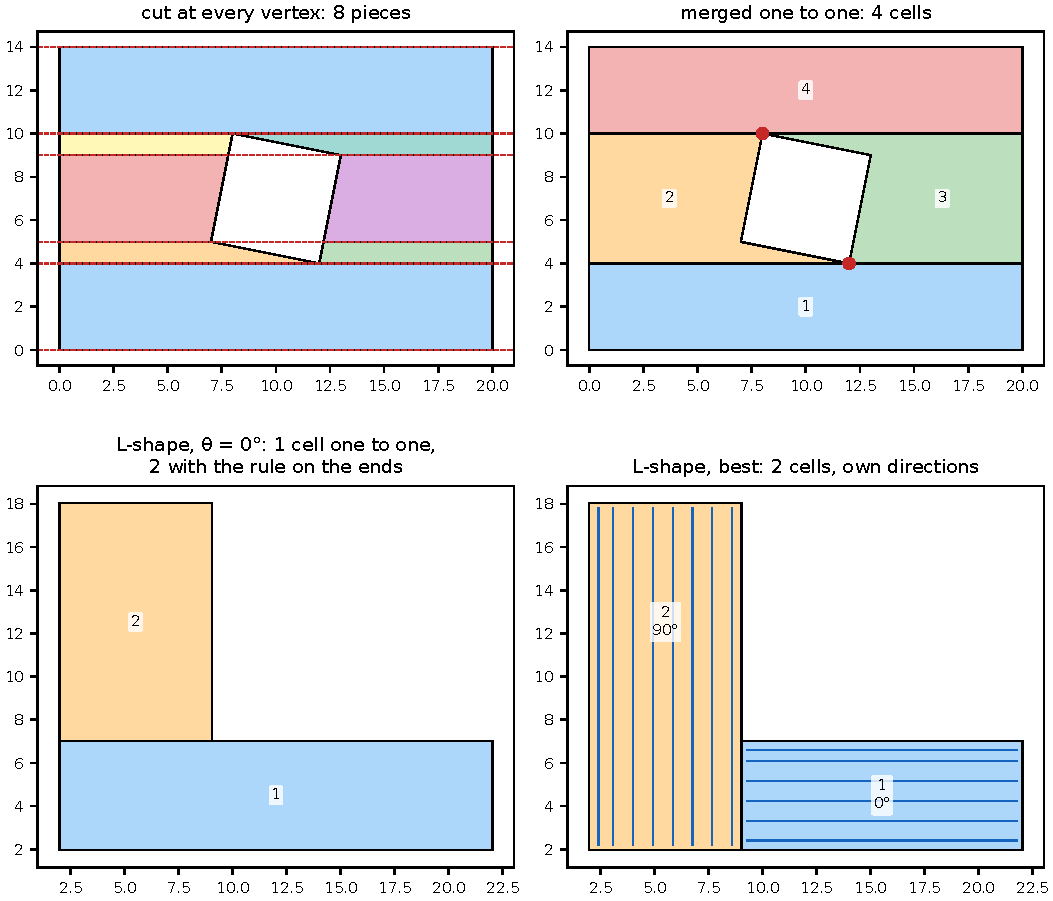
\includegraphics[width=\textwidth]{figures/decomposition}
  \caption{Top: a \SI{20}{\metre} by \SI{14}{\metre} region with a pond, cut
    by the horizontal lines through its vertices (dashed; red: through the
    vertices of the pond) into eight trapezoids, then merged into four
    monotone cells. The cuts left go through the critical points (red dots):
    there, a horizontal line goes from meeting the region once to meeting
    it twice. Bottom: the interior of the L-shape left by two headland
    passes. Left: with $\theta = 0$, one-to-one merging gives a single cell;
    the rule on the ends of the passes keeps the two arms apart. Right: the
    decomposition the planner keeps, the cut vertical and each cell with its
    own direction (blue: the swaths).}
  \label{fig:decomposition}
\end{figure}

\section{Keeping the ends of the passes in line}

The interior of the L-shape is monotone for $\theta = 0$, so the merge
gives a single cell (Figure~\ref{fig:decomposition}, bottom left). Yet the
passes of the lower arm end \SI{13}{\metre} further right than those of
the upper arm, and the order of the passes then mixes long and short
passes. The planner therefore adds a rule to the merge.

\begin{definition}{End jump}{endjump}
  Across a cut line, the \emph{end jump} between a cell $A$ below and a
  piece $B$ above is the larger of the distances between the left ends and
  between the right ends of the top side of $A$ and the bottom side of $B$.
  The planner merges $A$ and $B$ only if the end jump is at most
  \SI{1}{\metre}.
\end{definition}

On a curved border the pieces are thin and their ends move little from one
line to the next, so the cells still merge; at a corner of the border
parallel to the passes, the ends jump and a new cell starts. The L-shape
splits into its two arms.

\section{Choosing the cuts and the directions}

The decomposition depends on the direction of the sweep, and each cell can
then be mowed in its own direction, as long as it is monotone in that
direction. The planner tries the same candidate directions as in
Chapter~\ref{ch:swaths} (the edges of the convex hull and every $15°$),
and for each of them:

\begin{description}
  \item[Decomposes.]
    \leavevmode\\
    It cuts and merges as above, then merges cells smaller than $4w^2$
    (\SI{3.8}{\metre\squared}) into a neighbour when the union is still
    monotone in that neighbour's direction.
  \item[Chooses a direction per cell.]
    \leavevmode\\
    Among the candidate directions of the cell in which it is monotone, the
    one with the smallest estimated time (the estimate of
    Figure~\ref{fig:direction}).
  \item[Estimates the time.]
    \leavevmode\\
    The sum of the estimates of the cells, plus \SI{30}{\second} per cell
    for reaching it.
\end{description}

It keeps the decomposition with the smallest estimate. On the L-shape, it
cuts vertically: the upper arm and the part of the lower arm below it make
one cell of \SI{113.4}{\metre\squared}, mowed with vertical passes, and
the rest of the lower arm a cell of \SI{65.8}{\metre\squared}, with
horizontal passes (Figure~\ref{fig:decomposition}, bottom right). On the
garden it finds four cells (Figure~\ref{fig:gardencells}).

\begin{figure}[ht]
  \centering
  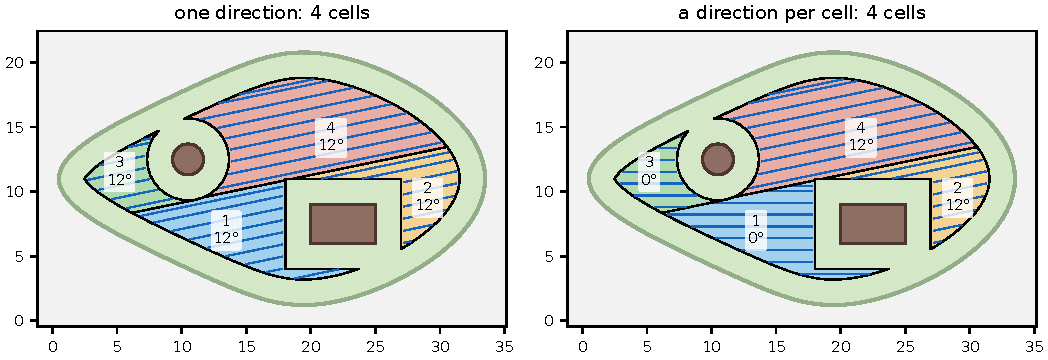
\includegraphics[width=\textwidth]{figures/garden_cells}
  \caption{The interior of the garden left by two headland passes, cut into
    cells (labels: the cell and the direction of its passes; blue: the
    swaths). Left: every cell mowed in the direction of the sweep. Right:
    each cell in its own best direction. The cuts start at critical points
    next to the two holes.}
  \label{fig:gardencells}
\end{figure}

\section{Mowing cell by cell}

The planner of this chapter mows the headland, then the cells one after
the other, each time the cell whose first or last swath has an end closest
to the mower. Each cell is mowed by the passes of Chapter~\ref{ch:swaths},
starting with the fastest of the four ways in, and the mower drives to the
next cell with the blades off. The order of the cells is greedy here;
Chapter~\ref{ch:order} improves it.

A pass may now end on a cut, inside the lawn, rather than on the headland.
The turn there runs over the neighbouring cell, which is lawn: the
collision checker accepts it, and the blades, engaged in turns, cut some of
that cell early.

\begin{figure}[ht]
  \centering
  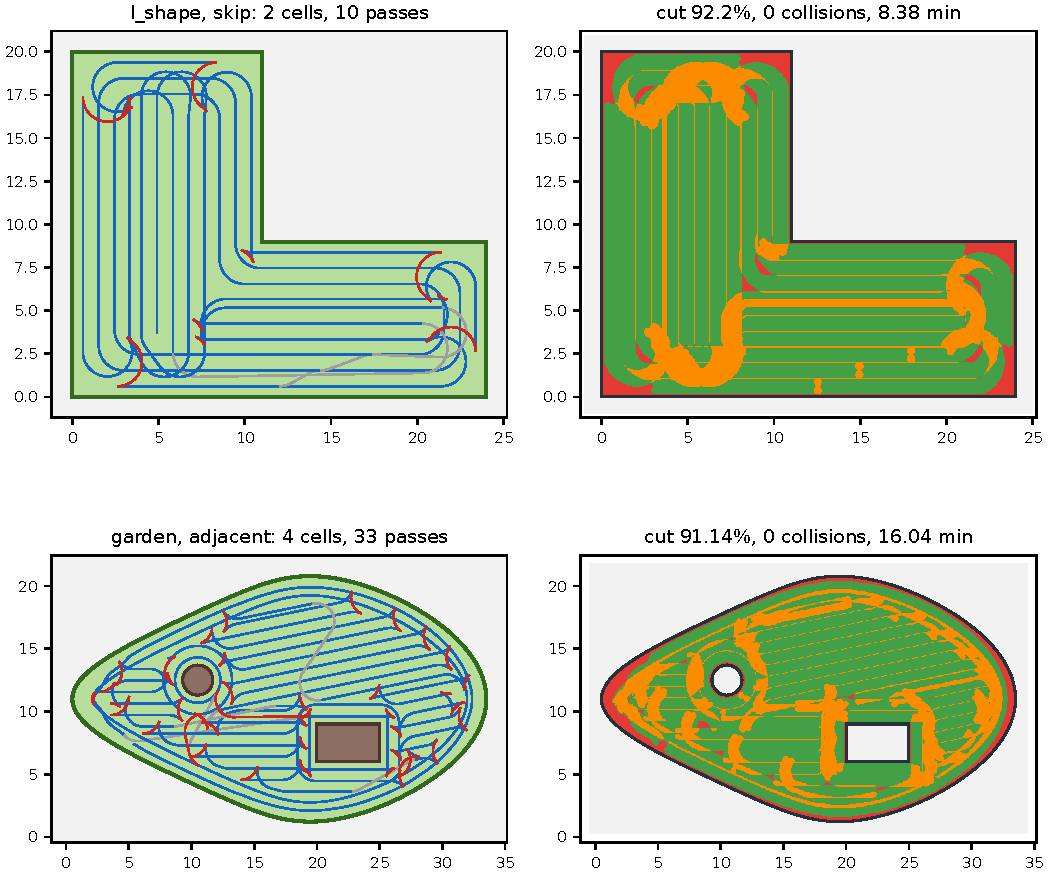
\includegraphics[width=\textwidth]{figures/cell_plans}
  \caption{Plans cell by cell. Top: the L-shape in two cells with the order
    with jumps (three headland passes); the vertical passes of the left
    cell turn in the headland at both ends. Bottom: the garden in four
    cells, passes in lateral order. Left: the path of the rear axle (blue
    forward, red reverse, grey blades off). Right: green cut once, orange
    twice, red missed.}
  \label{fig:cellplans}
\end{figure}

\begin{center}
\begin{tabular}{@{}llrrrrr@{}}
  \toprule
  lawn & order & cells & passes & cut & changes & time \\
  \midrule
  L-shape & adjacent & 2 & 14 & 93.0\% & 40 & \SI{9.11}{\minute} \\
  L-shape & skip & 2 & 10 & 92.2\% & 20 & \SI{8.38}{\minute} \\
  garden & adjacent & 4 & 33 & 91.1\% & 90 & \SI{16.04}{\minute} \\
  garden & skip & 4 & 24 & 90.6\% & 78 & \SI{15.78}{\minute} \\
  \bottomrule
\end{tabular}
\end{center}

On the L-shape the two cells save \SI{0.74}{\minute} over the single cell
of Chapter~\ref{ch:swaths} with the lateral order, and \SI{1.57}{\minute}
with the order with jumps (\SI{9.95}{\minute} there, \SI{8.38}{\minute}
here): with the ends of the passes in line, the jumps pay off again. The
rectangle is a single cell, and its plan is that of
Chapter~\ref{ch:swaths}. The garden is mowed for the first time
completely, with no collision, in about \SI{16}{\minute}; the
\SI{9}{\percent} missed are the strip along the border, the patch at its
sharp tip where the first ring is cut (Section~\ref{sec:corners}), and
thin gaps where cells meet the headland.

\begin{inwords}
  A complex lawn is cut into cells that each look like a simple lawn: lines
  parallel to the passes cross a cell once, and the passes of a cell end in
  line. The cuts start at the points where the border turns back, and at
  corners where the ends of the passes would jump. Each cell is then mowed
  in its own best direction.
\end{inwords}

\begin{incode}
  \code{mowersim/planning/cells.py}: \code{slices} (the cut),
  \code{decompose} (the merge, Propositions~\ref{prop:trapezoids}
  and~\ref{prop:merge}, with the end jump of Definition~\ref{def:endjump}),
  \code{is\_monotone}, \code{merge\_small}, \code{best\_cell\_direction},
  \code{best\_decomposition} and \code{plan\_cells}, the planner of this
  chapter.
\end{incode}
